\documentclass{article}

% if you need to pass options to natbib, use, e.g.:
%     \PassOptionsToPackage{numbers, compress}{natbib}
% before loading neurips_2018

% ready for submission
% \usepackage{neurips_2018}

% to compile a preprint version, e.g., for submission to arXiv, add add the
% [preprint] option:
%     \usepackage[preprint]{neurips_2018}

% to compile a camera-ready version, add the [final] option, e.g.:
     \usepackage[final]{nips_2018}

% to avoid loading the natbib package, add option nonatbib:
%     \usepackage[nonatbib]{neurips_2018}

\usepackage[utf8]{inputenc} % allow utf-8 input
\usepackage[T1]{fontenc}    % use 8-bit T1 fonts
\usepackage{hyperref}       % hyperlinks
\usepackage{url}            % simple URL typesetting
\usepackage{booktabs}       % professional-quality tables
\usepackage{amsfonts}       % blackboard math symbols
\usepackage{nicefrac}       % compact symbols for 1/2, etc.
\usepackage{microtype}      % microtypography
\usepackage{graphicx}
\usepackage{subcaption}

\graphicspath{ {imgs/} }

\title{CS 7180 Milestone 1}

% The \author macro works with any number of authors. There are two commands
% used to separate the names and addresses of multiple authors: \And and \AND.
%
% Using \And between authors leaves it to LaTeX to determine where to break the
% lines. Using \AND forces a line break at that point. So, if LaTeX puts 3 of 4
% authors names on the first line, and the last on the second line, try using
% \AND instead of \And before the third author name.

\author{%
  Nalin Gupta \\
  \texttt{gupta.nal@husky.neu.edu} \\
  \And
  Christopher Botica\\
  \texttt{botica.c@husky.neu.edu} \\
  \And
  Tyler Brown\\
  \texttt{brown.tyler@husky.neu.edu} \\
  % Coauthor \\
  % Affiliation \\
  % Address \\
  % \texttt{email} \\
  % \AND
  % Coauthor \\
  % Affiliation \\
  % Address \\
  % \texttt{email} \\
  % \And
  % Coauthor \\
  % Affiliation \\
  % Address \\
  % \texttt{email} \\
  % \And
  % Coauthor \\
  % Affiliation \\
  % Address \\
  % \texttt{email} \\
}

\begin{document}
% \nipsfinalcopy is no longer used

\maketitle

\section{Introduction and Related Work}

Images taken in low-light conditions are often too dark, noisy, and distorted to be used in industrial purposes. We propose a deep-learning model that processes low-light
images to improve image brightness and increase their overall quality.

The problem with imaging in low-light conditions is challenging due to low-photon count
and low Signal-to-Noise (SNR) ratio. These yield very dark and noisy images.
The most common technique to overcome this problem is long exposure shot.
However, this method yields blurry images with the slightest camera shake
or object motion\cite{chen2018learning}. Common post-processing techniques brighten the image at the expense of image quality. 

Being able to ``see in the dark'' provides a
number of real-world benefits such as photography, computer vision, and
social networking. 

In the past, the problem of enhancing low light images has been tackled via
noise reduction. This noise becomes dominant especially in low-light images
due to low SNR. Remez et. al. proposed a deep CNN for noise reduction under
the assumption that this low-light noise belongs to a Poisson
distribution \cite{remez2017deep}.  They used images from ImageNet
\cite{imagenet_cvpr09} as their ground truth data
and added synthetic Poisson noise to simulate corrupted images. Even though
their model outperform the state-of-the art de-noiser ``BM3D'', it does not
scale well to real world images, due to their underlying assumptions.
Furthermore, their model only denoises images but does not brighten them.
Motivated by these downfalls, Chen et. al., proposed an end-to-end CNN,
``See-in-the-Dark'' (SID), which brightens extremely low light images and
removes noise without making any underlying assumptions
\cite{chen2018learning}. However these advances come with the added expense
of collecting large amounts of low
light and bright light images. In the absence of a true vs noisy image
dataset, the team captured scenes using various exposure times to generate
true (bright light) and corrupted (low light) image pairs called
``See-in-the-Dark Dataset'' (SID Dataset \footnote{https://github.com/cchen156/Learning-to-See-in-the-Dark}). Furthermore, their model is camera
specific and not easily generalizable.

We propose a transferable CNN for image brightening and denoising. Instead
of training our model on actual true (bright light) and corrupted
(low light) image pairs, we use images from the publicly available "MIT-Adobe FiveK Dataset" dataset as our baseline and corrupt these by simulating low-light conditions. We train our CNN on the synthetic data to obtain our initial model
parameters. Then, using these, and a small fraction of the real image pairs
from the SID Dataset, we adopt a transfer learning
\cite{Goodfellow-et-al-2016} approach to update our
model parameters. We then use this model to test on our SID Dataset. In
addition, we aim to test various transfer learning approaches, such as the
traditional transfer learning and zero shot learning \cite{larochelle2008,
  Palatucci:2009:ZLS:2984093.2984252, socher2013zeroshot}.


The novelty of our approach stems from the idea of ``more for less''. Our
model drastically reduces the overhead costs of data collection by
synthesizing readily available training data (MIT-Adobe FiveK). This is
particularly beneficial in domains where collecting images pairs is
expensive/time consuming. 


We use the SID Model as our baseline and our performance measure will be achieving a Peak Signal-to-Noise Ratio (PSNR) greater or equal to the baseline.

\section{Model}

We first collect 5,000 images in raw format from the MIT-Adobe dataset, taken with SLR camers by a set of different photographers in different scenarios. We made sure that these photographs cover a broad range of scenes, subjects, and lighting conditions. 

Considering these images as the ground truth (i.e., images taken in normal light conditions), we corrupt them to simulate images taken in low-light conditions. These distorted images and original images consist of our training inputs to our first model. 
In order to simulate the distortion created by taking pictures in poor light conditions, we emulate the traditional image processing pipeline for correcting such images, only in reverse. 

As illustrated in Figure 1, the traditional pipeline takes a corrupted image, and applies the following sequence of modules: Reduce Black Level, Denoising, White Balance, and Gamma Correction. The Black Level refers to refers to the level of brightness at the darkest parts of the image, and is reduced by subtracting the minimum pixel value. Denoising is reduced using common algorithms such as BM3D. White Balance refers to the color balance in the image (i.e., white should be true white) and is corrected by re-balancing the intensities of each color RGB. Finally, Gamma Correction controls the overall brightness of the image. We synthetically generate corrupted images by applying the reverse of this pipeline. Gamma Distortion: decrease the brightness of the image during our Gamma Distortion step, White Imbalance: skew the color-space by multiplying each level of RGB by a random weight, Poisson Noise: add Poisson noise to the image, Black Level: add a positive bias to the pixel values (i.e., random black level). 

\begin{figure}[ht]
  \centering
  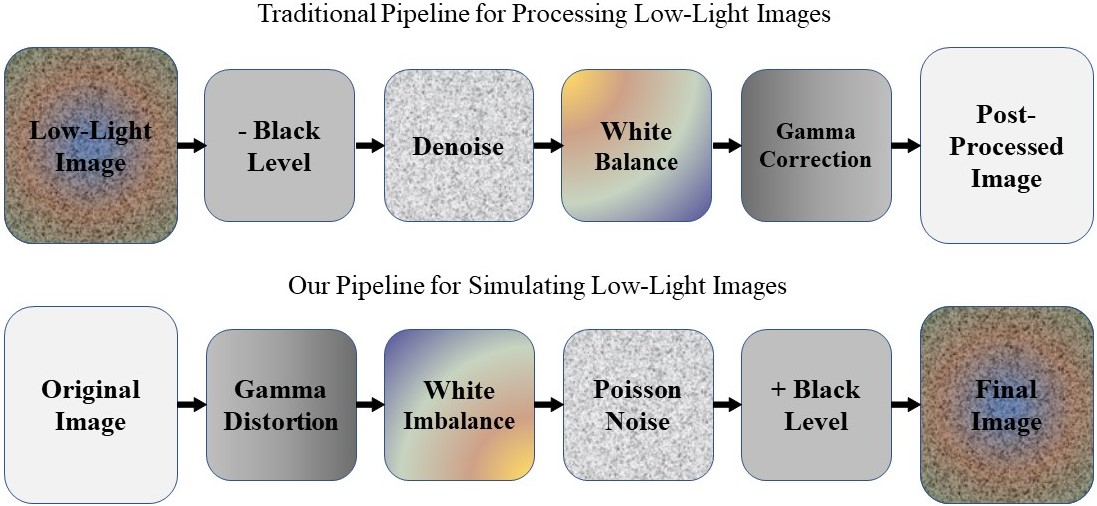
\includegraphics[scale=0.35]{pipeline.jpg}
  \caption{Top: Traditional Pipeline for processing low-light images. Bottom: Our  pipeline to simulate low-light images based on the traditional, only in reverse.}
\end{figure}


Our model is based on the one developed for SID, with the addition of 2 fully-connected layers. Note that we may increase this if training runtime permits. Using the transfer learning approach, we will first train our model on the MIT dataset, then erase the learned weights from the last two fully-connected layers, and retrain on the SID dataset. This is highlighted in our model framework in Figure 2. 

\begin{figure}[ht]
  \centering
  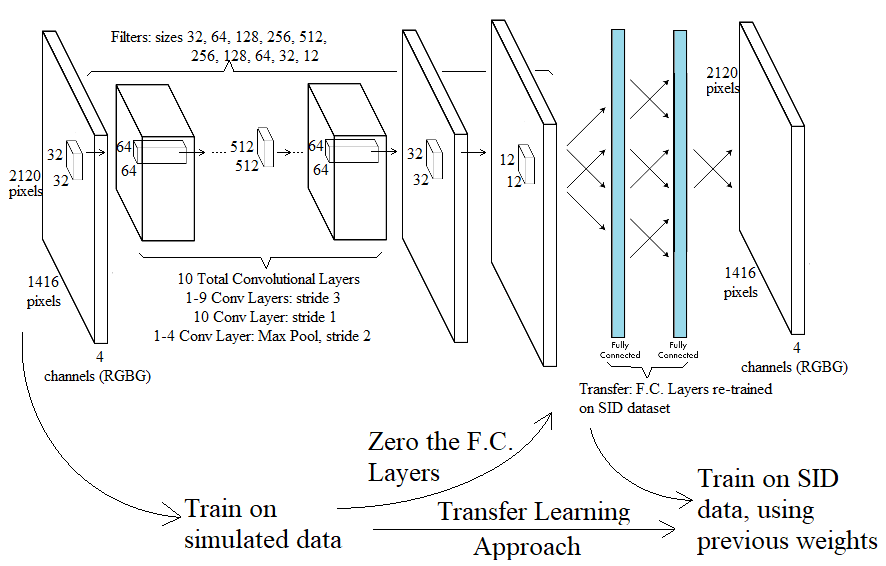
\includegraphics[scale=0.3]{model.png}
  \caption{Our proposed model framework}
\end{figure}



\section{Experiment}

We first collect 5,000 images in raw format from the MIT-Adobe dataset, taken with SLR cameras by a set of different photographers in different scenarios. We then run these images through our pipeline to generate our simulated low-light images. An example of two of such images is represented in Figure 3. 

\begin{figure}[ht]
  \centering
  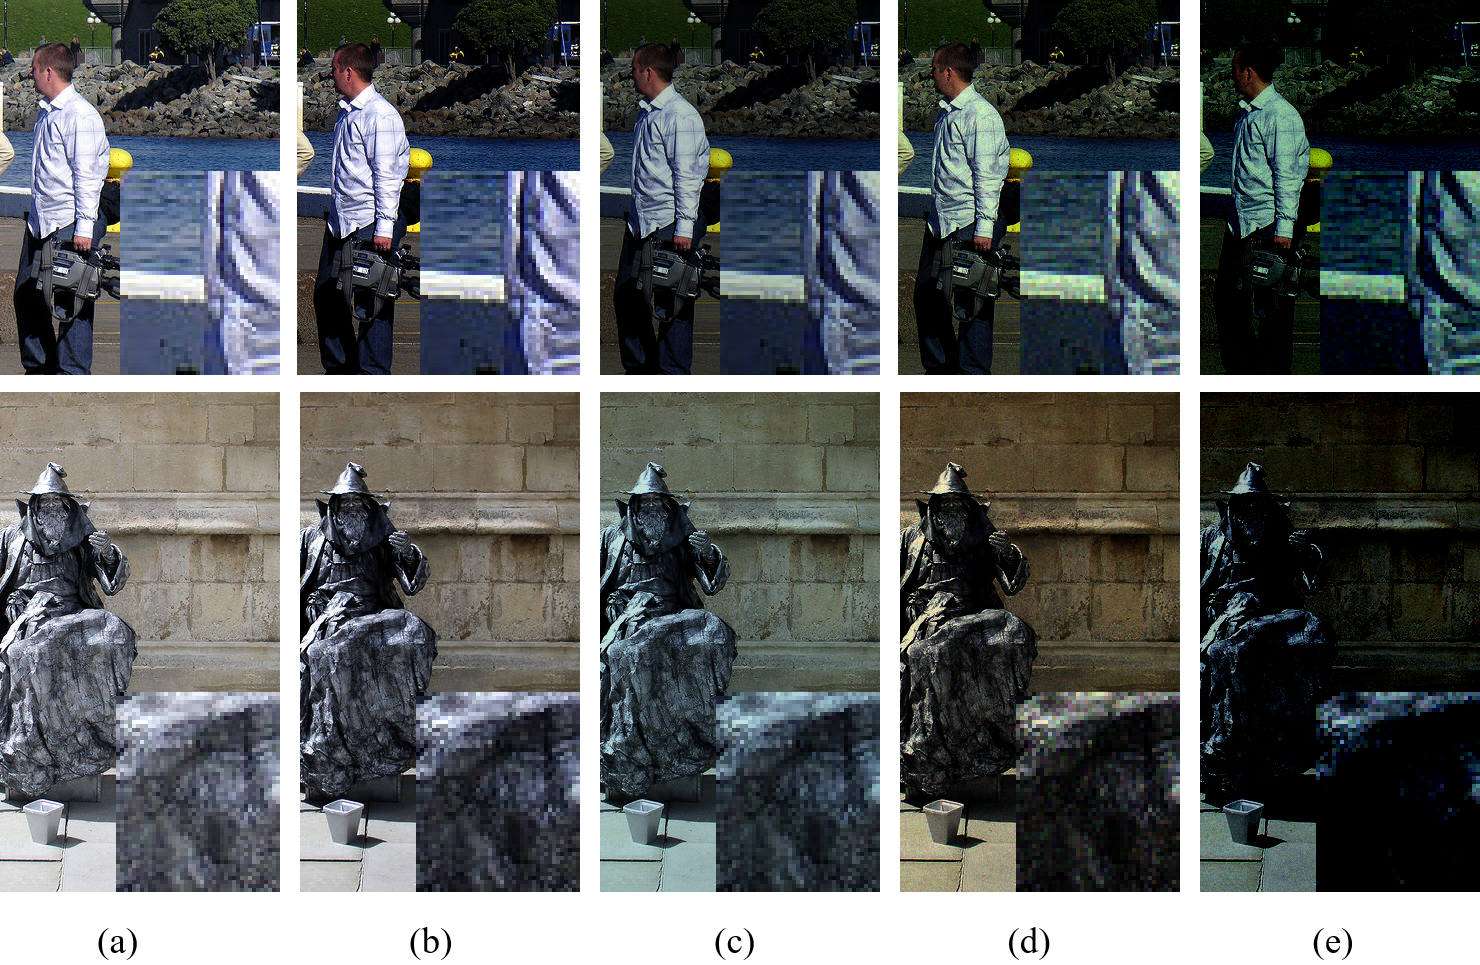
\includegraphics[scale=0.3]{fig3.png}
  \caption{Simulating two low-light images via our pipeline: (a) Gamma Distortion, (b) White Imbalance, (c) Poisson Noise addition, (d) Black Level, (e) Final low-light simulation}
\end{figure}

We use the SID Model as our baseline and our performance measure will be achieving a Peak Signal-to-Noise Ratio (PSNR) greater or equal to the baseline.

Using the GitHub repository provided by Chen et. al. \cite{chen2018learning},
we were gather and run to run their code but ran into limitations with computational
resources. Chen et. al. \cite{chen2018learning} used a separate model for
each of the two cameras. They specified a minimum of 64GB of GPU RAM for the
Sony model and 128 GB of GPU RAM for the Fuji model. We decided to try
replicating the less resource intensive Sony model. The hardware
requirements for the Sony model are nontrivial so we have explored
several options.

\begin{enumerate}
\item Using AWSEducate did not work
  \begin{itemize}
    \item Unable to create roles with IAM authentication so it's really
	 hard or impossible to move data from a S3 Bucket to an EC2 Instance
    \item Tried to create a $p3.8xlarge$ instance but these instances are
      not allowed even though they are listed
  \end{itemize}
\item Using regular AWS does work but is costly
  \begin{itemize}
    \item Ran a single AWS EC2 $p3.8xlarge$ instance with 32 CPU, 244 GB of
	 Memory, 4 Tesla V100 GPUs, and 64 GPU Memory. This costs \$12.24
	 an hour.
    \item This is the amount of GPU Memory requested by the paper
      authors as a minimum amount
    \end{itemize}
\end{enumerate}

Given these initial facts, we then tried to estimate run time requirements
for the Sony model. We trained the Sony model for 90 minutes using an
AWS $p3.8xlarge$ instance. We were able to complete $\approx 12$ training
epochs. Figure \ref{train} contains an example test image/labelled image
pairing. We then tried to use the training parameters to
test the model but could not get this to work without modifying the script
provided by Chen et. al. \cite{chen2018learning}. The model parameters
were available to download, we used these parameters to run against test
data for 30 minutes. Figure \ref{test} contains example output from this
test run. Both Figure \ref{train} and Figure \ref{test}
are pictures of a similar yellow bike. We can see a qualitative improvement
across the three renderings of the same predicted test image in
Figure \ref{test}.

Additional time was required to extract the Sony dataset
which decompressed to about 115GB of image files. We estimate that
replicating the Chen et. al. \cite{chen2018learning} training parameters
for \textit{only} the Sony model takes approximately 500 hours or
\$ 6,120.

\section{Appendix}

\begin{figure}[ht]
  \centering
  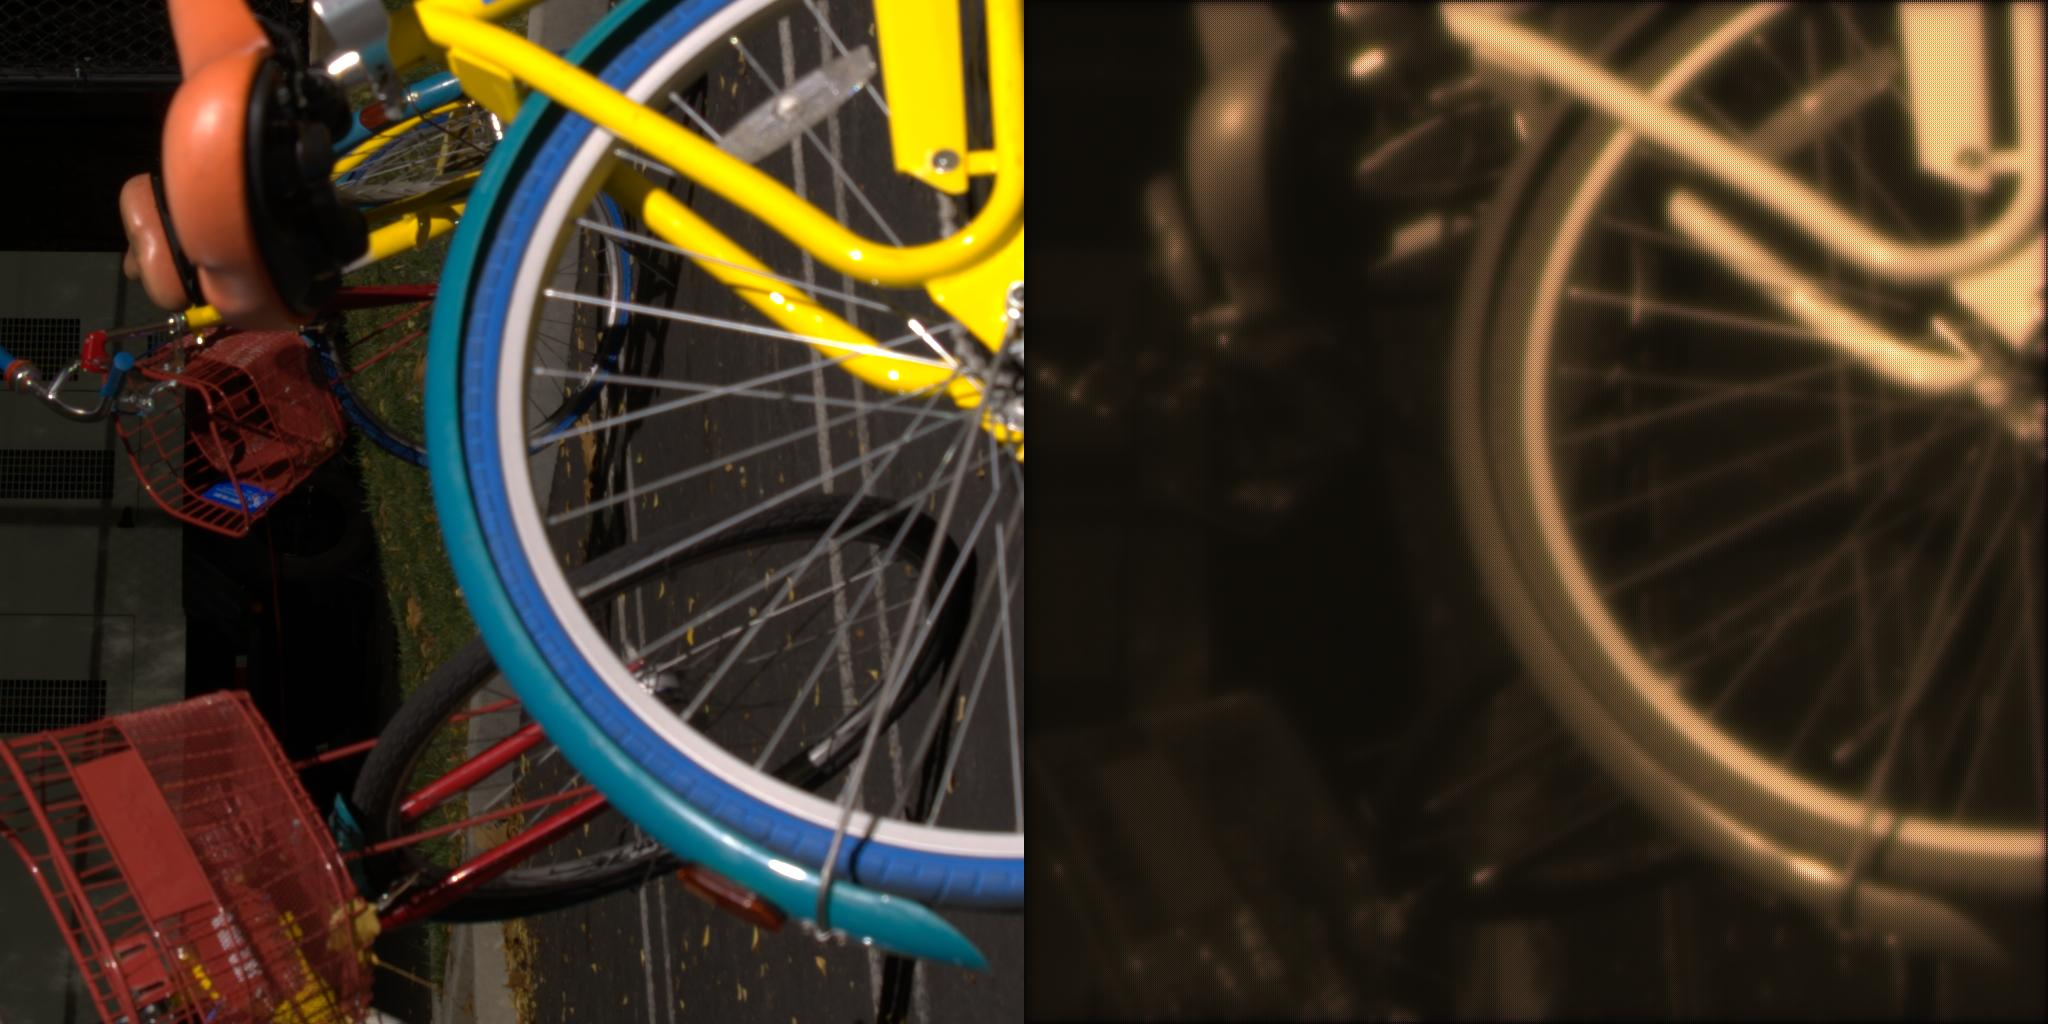
\includegraphics[scale=0.1]{00002_00_train_100}
  \caption{\label{train} Example Training Data}
\end{figure}


\bibliographystyle{unsrt}
\bibliography{references}

\end{document}
